\documentclass[../main.tex]{subfiles}

\begin{document}

The alignment operation is a long-running operation, possibly taking several dozens of minutes, in some cases even exceeding an hour. Hence, there is no doubt that this operation has to be asynchronous.

In essence, everything depicted in Figure \ref{fig:alignment-process} as Reqour's responsibility is delegated to an Adjuster, which is created per alignment (hence per build) inside the corresponding PNC OpenShift cluster.

The endpoint handler itself is being pretty simple: asynchronously starts execution of some code (in this case creation of Adjuster Job in the OpenShift cluster) and immediately returns 202 Accepted.

Once the created Adjuster is fully initialized, all the work is done in there: optionally synchronize the downstream repository to the upstream repository, clone the source code from the downstream repository, start a manipulator (as \textit{java -jar manipulator.jar})\footnote{The only difference is SMEG which is distributed as an SBT plugin, thus being run directly through SBT.} communicating with DA during the alignment process, and make a callback at the end.

The above word description is visualized in Figure \ref{fig:alignment-design}.

\textbf{Note:} Even though Adjuster is depicted to be created in a separate OpenShift cluster, in fact, all the PNC microservices in the Figure (BPM, DA, Adjuster) are within the very same cluster (actually, even within the very same namespace).

\begin{figure}
  \begin{center}
    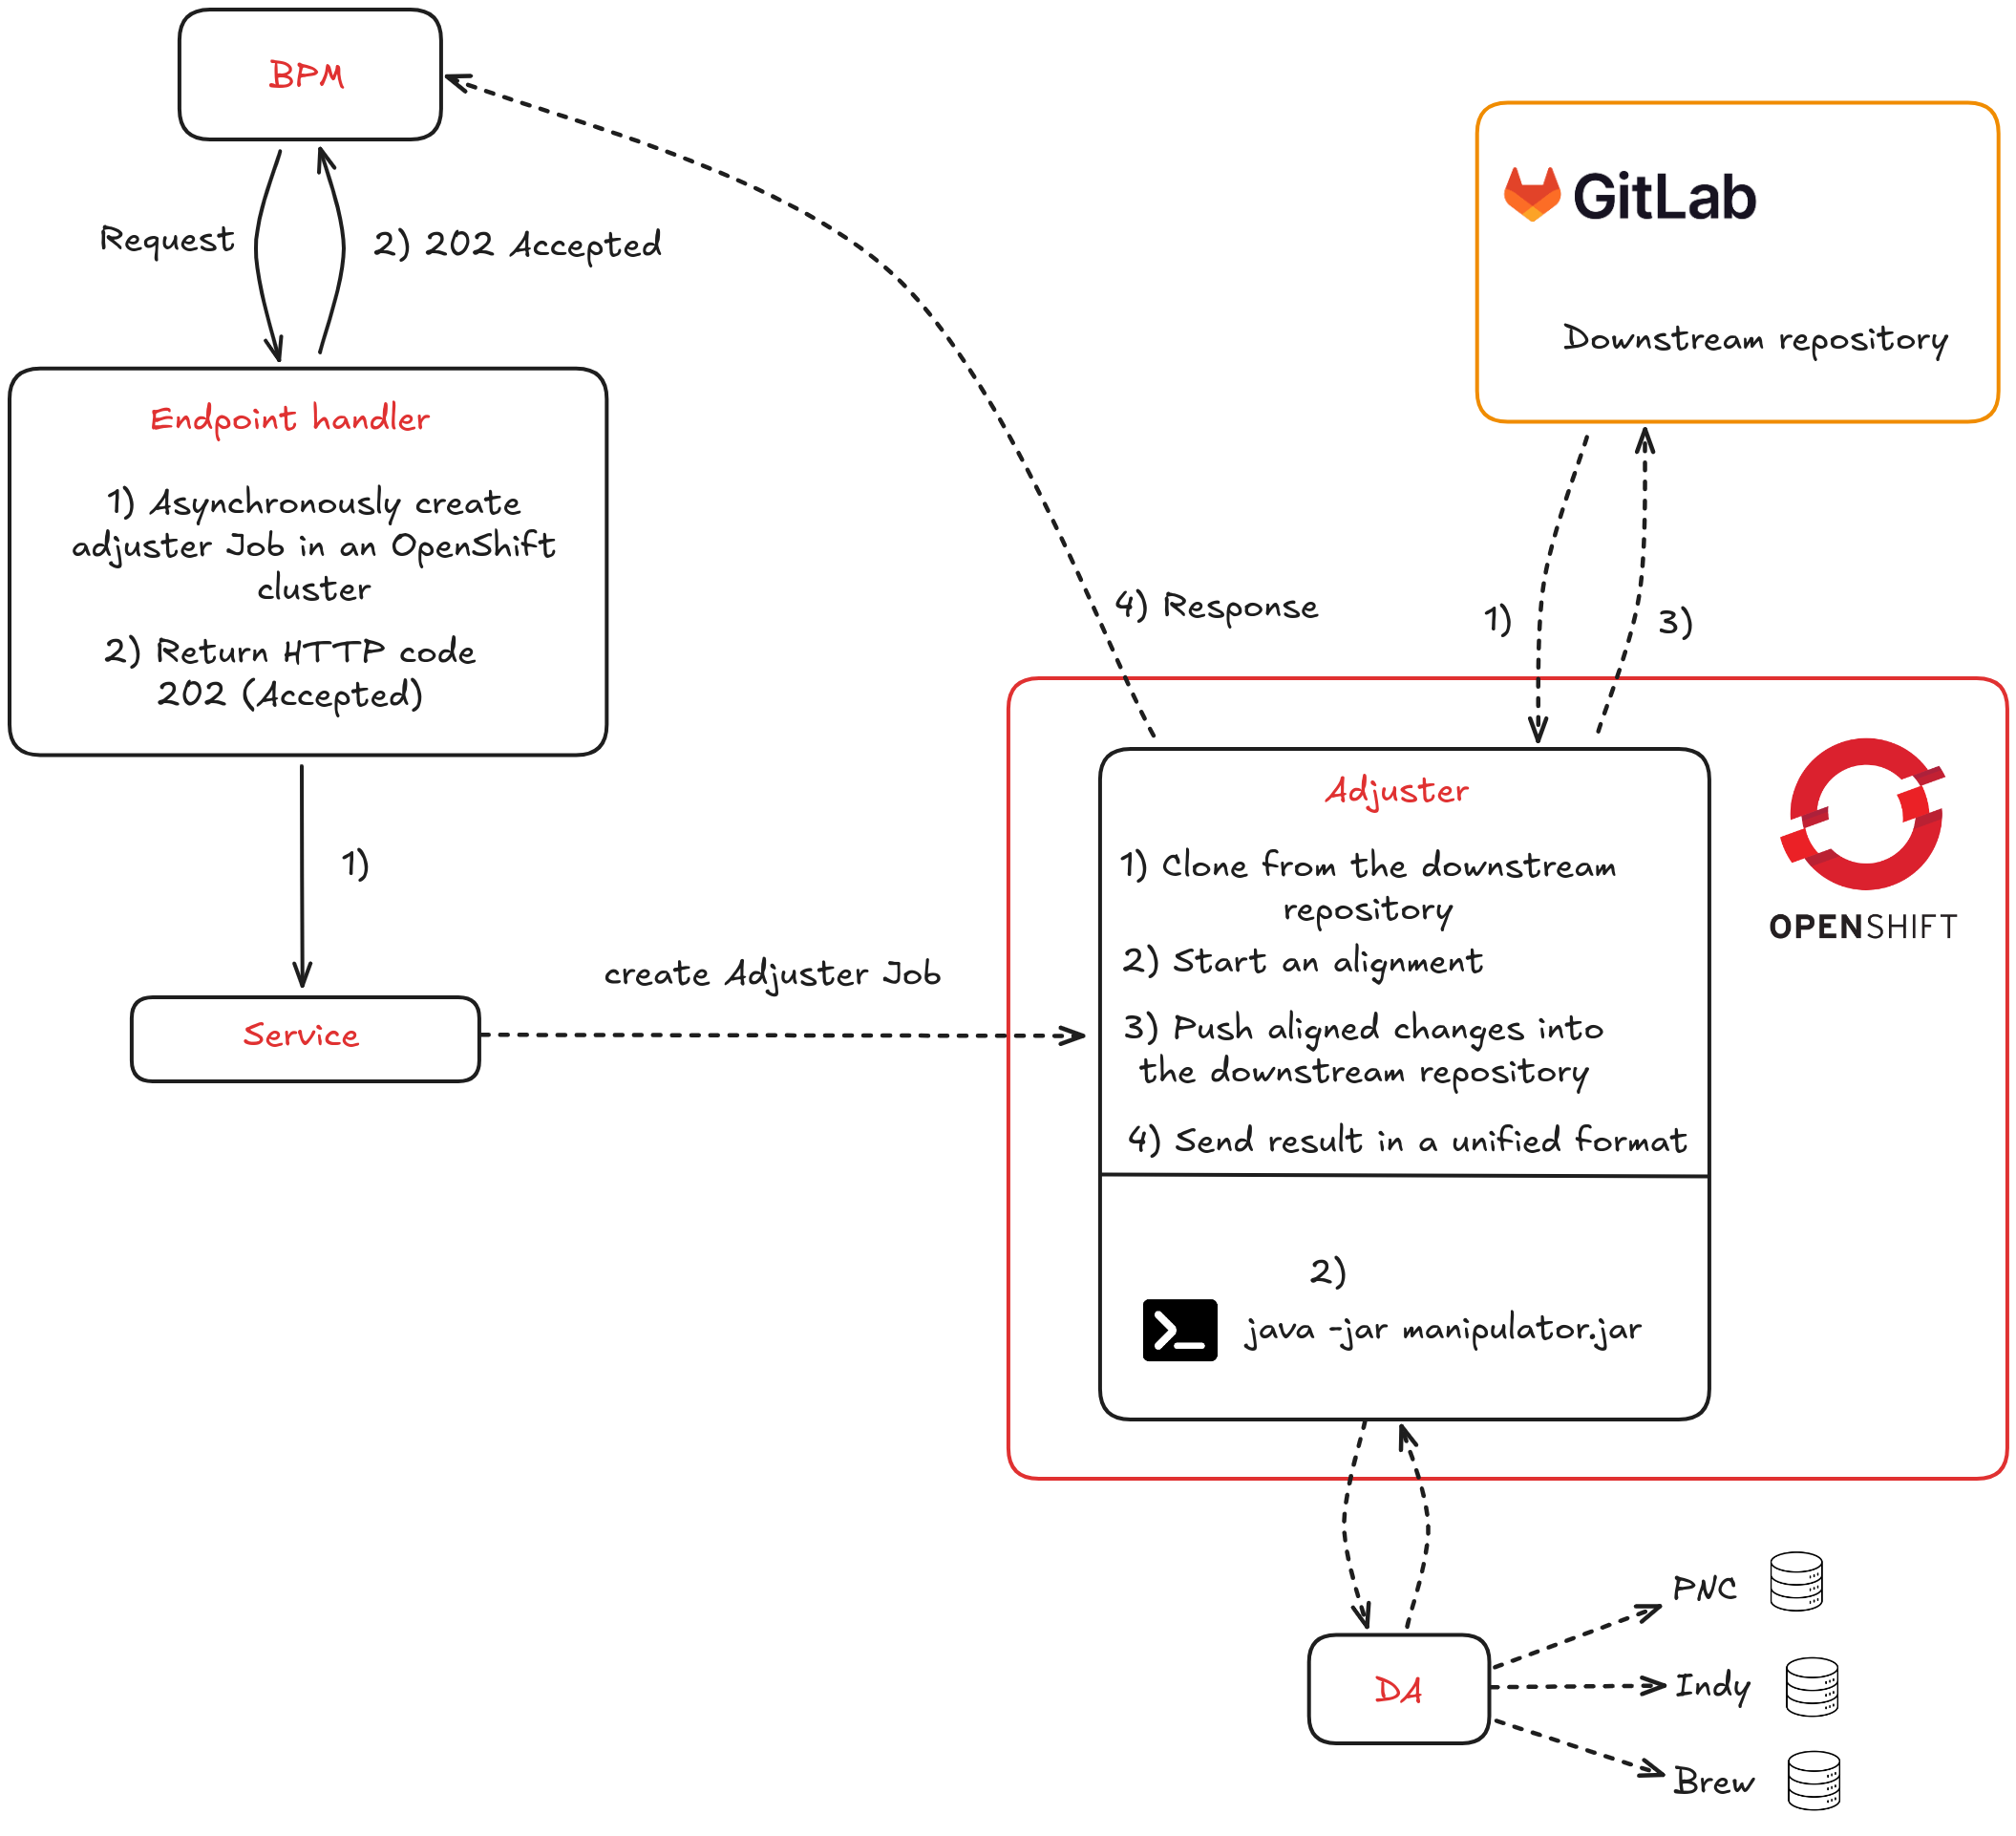
\includegraphics[width=\textwidth]{images/alignment-design.png}
  \end{center}
  \caption{Design of the alignment operation}
  \label{fig:alignment-design}
\end{figure}

\end{document}
